\documentclass[10pt,letterpaper]{article}
\usepackage[lmargin=2.2in,rmargin=0.7in,tmargin=1.0in,bmargin=1.0in]{geometry}
\usepackage{notes}
\begin{document}

\begin{center}
\Large\textbf{2.7 -- Forced Springs: Beats and Resonance}\\
\normalsize (Section 2.3.2)
\end{center}


%%%%%%%%%%%%%%%%%%%%%%%%%%%%%%%%%%%%

\section{Forced Vibrations with Damping}

\subsection{Spring-Mass System}

A spring-mass system driven by an external force satisfies
\[
\underbrace{mx''}_{\text{inertia}}
+\underbrace{\gamma x'}_{\text{damping}}
+\underbrace{kx}_{\text{restoring}}
=\underbrace{f(t)}_{\text{external}}.
\]
Each term represents a force. We focus on sinusoidal forcing,
\[
f(t)=F_0\cos(\omega t),
\]
where $F_0$ is the force amplitude in newtons and $\omega$
is the \textbf{forcing frequency}. A motorized piston
moving the spring's attachment point back and forth
can produce this type of forcing.

\begin{figure}[H]
\centering
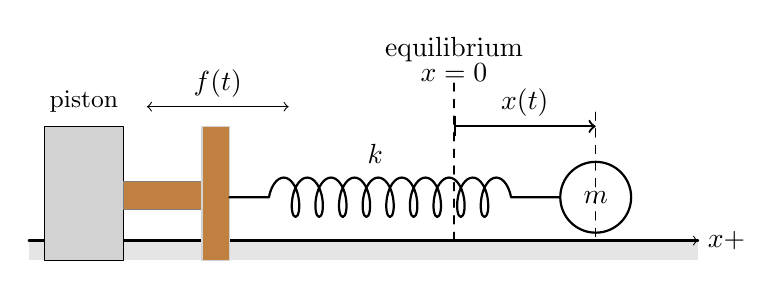
\begin{tikzpicture}[scale=1.0,line cap=round,line join=round]
    % Requires decorations.pathmorphing in the preamble
    \def\wallX{2}
    \def\eqX{5.2}
    \def\massX{7.0}
    \def\massR{0.45}
    \def\springY{0.55}

    % Table
    \fill[gray!20] (-0.2,-0.25) rectangle (8.3,0);
    \draw[thick] (-0.2,0) -- (8.3,0);
    \draw[->] (0,0) -- (8.3,0) node[right] {$x+$};

    % Piston and moving attachment
    \draw[fill=gray!35] (0,-0.25) rectangle (1,1.45);
    \draw[fill=brown,draw=gray]
        (1,0.4) rectangle (2,0.75);
    \draw[fill=brown,draw=gray!35]
        (\wallX,-0.25) rectangle (\wallX+0.35,1.45);
    \node[above] at (0.5,1.5) {\small piston};
    \draw[<->] (1.3,1.7) -- (3.1,1.7);
    \node at (2.2,2) {$f(t)$};

    % Coiled spring
    \draw[
        thick,
        decorate,
        decoration={
            coil,
            aspect=0.45,
            amplitude=2.5mm,
            segment length=3mm,
            pre length=5mm,
            post length=4mm
        }
    ]
        (\wallX+0.35,\springY)
        -- (\massX-\massR,\springY);
    \node[above] at (\wallX+2.2,\springY+0.30) {$k$};

    % Reference equilibrium
    \draw[dashed] (\eqX,0) -- (\eqX,2.0);
    \node[above] at (\eqX,2.15) {equilibrium};
    \node[above] at (\eqX,1.9) {$x=0$};

    % Mass
    \draw[thick,fill=white]
        (\massX,\springY) circle (\massR);
    \node at (\massX,\springY) {$m$};

    % Displacement
    \draw[dashed]
        (\massX,\springY-\massR-0.05)
        -- (\massX,\springY+\massR+0.65);
    \draw[|->,thick]
        (\eqX,\springY+\massR+0.45)
        -- (\massX,\springY+\massR+0.45);
    \node[above]
        at ({(\eqX+\massX)/2},\springY+\massR+0.45)
        {$x(t)$};
\end{tikzpicture}
\caption{A motorized piston drives the spring-mass system.
Displacement is measured from the equilibrium position
with the piston at its reference position.}
\end{figure}

%-------------------------------------------------------------
\subsection{Levels of Specificity}

Recall that nonhomogeneous solutions have the form $x=x_h+x_p$. Depending on the question,
we may need only the form of these pieces or their exact
coefficients. For example, consider
\[
x''+2x'+5x=25t,\qquad x(0)=0,\quad x'(0)=5.
\]
\begin{enumerate}
    \item \textbf{General form}: find $x_h$ and choose a trial
    for $x_p$, leaving its coefficients undetermined:
    \[
    x=e^{-t}(c_1\cos2t+c_2\sin2t)+At+B.
    \]

    \item \textbf{General solution}: determine $A$ and $B$
    by substitution:
    \[
    x=e^{-t}(c_1\cos2t+c_2\sin2t)+5t-2.
    \]

    \item \textbf{Solution to the IVP}: use the initial
    conditions to determine $c_1$ and $c_2$:
    \[
    x=e^{-t}(2\cos2t+\sin2t)+5t-2.
    \]
\end{enumerate}
In this lecture, we mainly use the \textbf{general form}
to predict behavior without calculating every coefficient.

%-------------------------------------------------------------
\begin{example}[1]{
A spring-mass system has mass $m=1$ kg, damping coefficient
$\gamma=3$ kg/s, and spring constant $k=2$ N/m.
An external force $f(t)=10\cos t$ N acts on the mass.
Initially, the mass is displaced $30$ cm to the right
and given a rightward velocity of $1$ m/s.

Formulate the IVP and find the general form of the solution.
Do not determine the coefficients.
}
Substituting into $mx''+\gamma x'+kx=f(t)$ gives $x''+3x'+2x=10\cos t,$. We treat displacement to the right of the equilibrium as positive. So the displacement $30$ cm $= 0.3$ m is written $x(0)=0.3$. Our model is
\[
\begin{dcases}
x''+3x'+2x=10\cos t,\\
x(0)=0.3,\\
x'(0)=1.
\end{dcases}
\]
The characteristic equation is
\[
\lambda^2+3\lambda+2=(\lambda+1)(\lambda+2)=0,
\]
so $x_h(t)=c_1e^{-t}+c_2e^{-2t}$.
For the forcing term, choose
$x_p(t)=A\cos t+B\sin t$. There is no duplication,
so the general form is
\[
\boxed{
x(t)=
\underbrace{c_1e^{-t}+c_2e^{-2t}}_{\text{decays}}
+
\underbrace{A\cos t+B\sin t}_{\text{persists}}.
}
\]
Without finding the coefficients, we can already see
that the exponential terms vanish and the sinusoidal
part remains. Although the system is \textbf{overdamped},
periodic forcing keeps it oscillating. For illustration, the graph shows the solution after
the coefficients have been determined.

\begin{center}
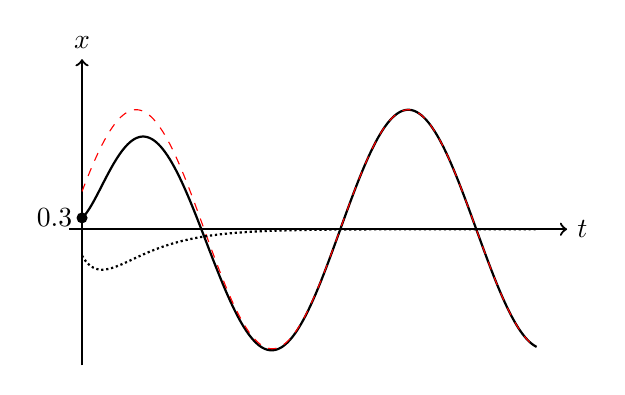
\begin{tikzpicture}[x=0.55cm,y=0.48cm]
    \def\xMax{10.5}

    % Axes
    \draw[->,thick] (-0.3,0) -- (11.2,0)
        node[right] {$t$};
    \draw[->,thick] (0,-3.6) -- (0,4.5)
        node[above] {$x$};

    % Full solution
    \draw[thick,domain=0:\xMax,samples=400]
        plot (\x,{
            cos(deg(\x))+3*sin(deg(\x))
            -3.4*exp(-\x)+2.7*exp(-2*\x)
        });

    % Persistent part
    \draw[red,dashed,domain=0:\xMax,samples=400]
        plot (\x,{cos(deg(\x))+3*sin(deg(\x))});

    % Decaying part
    \draw[densely dotted,thick,domain=0:\xMax,samples=200]
        plot (\x,{-3.4*exp(-\x)+2.7*exp(-2*\x)});

    % Initial displacement
    \fill (0,0.3) circle (2pt);
    \node[left] at (0,0.3) {$0.3$};
\end{tikzpicture}

\small
Solid: full solution.
Dashed: persistent part.
Dotted: decaying part.
\end{center}
\end{example}

%-------------------------------------------------------------
\subsection{Transient vs. Steady-State Solution}

The two behaviors in Example 1 have names. For a model with forced vibrations and damping, the solution has the general form
\[
x(t)=
\underbrace{x_h(t)}_{\text{transient}}
+
\underbrace{A\cos(\omega t)+B\sin(\omega t)}_{\text{steady-state}}.
\]
The \textbf{transient solution} $x_h$ is a short-lived function which decays to zero
due to the friction in the system. The sinusoidal particular solution
is the \textbf{steady-state solution}. The transient solution captures the contribution from the initial conditions, while the steady-state solution captures the response to the forced vibration.

We will always obtain transient and steady state solutions from the model
\[
mx''+\gamma x'+kx
=F_0\cos(\omega t),
\]
if $\gamma\ne0$. If $\gamma =0$, then we may obtain more interesting solutions.

% -----------------
% \subsection{RLC Circuit}

% The charge $Q(t)$ on the capacitor in a series
% \textbf{RLC circuit} satisfies
% \[
% LQ''+RQ'+\frac{1}{C}Q=E(t),
% \]
% where $L>0$ is inductance, $R>0$ is resistance, $C>0$ is
% capacitance, and $E(t)$ is the applied voltage.
% The current is $I(t)=Q'(t)$. This has the same form as the spring-mass equation:
% \[
% L\leftrightarrow m,\qquad
% R\leftrightarrow \gamma,\qquad
% \frac{1}{C}\leftrightarrow k,\qquad
% E(t)\leftrightarrow f(t).
% \]
% Resistance acts like damping, while the applied voltage
% acts like an external force. A sinusoidal voltage source
% has the form $$E(t)=F_0\cos(\omega t).$$ 
% \begin{figure}[H]
% \centering
% \begin{circuitikz}[american currents, american voltages]
%   % Main loop
%   \draw
%   (0,0) to[short]      (1,0)
%         to[sV,l=$E(t)$] (2,0)
%         to[short]      (3,0) 
%         to[closing switch,l=switch] (4,0)
%         to[short] (5,0)  % bottom left corner 
%         to[short] (5,1)
%         to[inductor,l=$L$] (5,2)
%         to[short] (5,3) % top right corner 
%         to[capacitor,l=$C$] (0.3,3)
%         to[short] (0,3) % top left corner
%         to[short] (0,2)
%         to[resistor,l=$R$] (0,1)
%         to[short] (0,0)
%         ;
% \end{circuitikz}
% \caption{A series RLC circuit driven by an applied voltage
% $E(t)$, analogous to a spring driven by an external force.}
% \end{figure}

% -------------------

%%%%%%%%%%%%%%%%%%%%%%%%%%%%%%%%%%%%
\section{Forced Vibrations without Damping}

\subsection{Natural and Forcing Frequencies}

If we assume that friction is negligibly small $(\gamma=0)$, then our model for a spring driven by a sinusoidal force satisfies
\[
mx''+kx=F_0\cos(\omega t).
\]
Dividing by $m$ gives
\[
x''+\omega_0^2x=F\cos(\omega t),
\qquad
\omega_0=\sqrt{\frac{k}{m}},
\qquad
F=\frac{F_0}{m}.
\]
There are two angular frequencies to distinguish:
\begin{itemize}
    \item $\omega_0$: the \textbf{natural frequency},
    determined by the mass and spring constant.
    \item $\omega$: the \textbf{forcing frequency},
    determined by the external source.
\end{itemize}
The homogeneous solution (solution to $x''+\omega_0^2x=0$) is
\[
x_h(t)=c_1\cos(\omega_0t)+c_2\sin(\omega_0t).
\]
In the absence of an external force, the spring oscillates according to the natural frequency $\omega_0$. Since we assume there is no friction, the homogeneous solution does not vanish.

%-------------------------------------------------------------
\subsection{Three Cases}

The relationship between the two frequencies determines
the behavior:
\begin{enumerate}
    \item \textbf{Far apart}: a fast wave combines with
    a slow wave.
    \item \textbf{Close but unequal}: waves of comparable
    amplitude produce \textbf{beats}.
    \item \textbf{Equal}: nonzero sinusoidal forcing
    produces \textbf{resonance}, with unbounded growth.
\end{enumerate}

%-------------------------------------------------------------
\subsection{Distinct Frequencies}

If $\omega\ne\omega_0$, the trial function
\[
x_p(t)=A\cos(\omega t)+B\sin(\omega t)
\]
does not overlap with $x_h$. Thus, the general form is
\[
x(t)=c_1\cos(\omega_0t)+c_2\sin(\omega_0t)
+A\cos(\omega t)+B\sin(\omega t).
\]
We can already see that the solution is bounded:
it is a sum of waves with constant coefficients.

%-------------------------------------------------------------
\begin{example}[2]{
Find the general form of the solution to
\[
x''+100x=99\cos t.
\]
}
The characteristic roots are $\lambda=\pm10i$, so
$\omega_0=10$. The forcing frequency is $\omega=1$.
There is no duplication, giving
\[
\boxed{
x(t)=c_1\cos10t+c_2\sin10t+A\cos t+B\sin t.
}
\]
The motion combines waves with frequencies $10$ and $1$.
\end{example}

%-------------------------------------------------------------
%-------------------------------------------------------------
\subsection{Interference}

Adding waves produces \textbf{interference}: they reinforce
one another when they have the same sign and partially
or completely cancel when they have opposite signs. To illustrate, take the solution from Example 2 with
$c_1=A=1$ and $c_2=B=0$:
\[
x(t)=
\underbrace{\cos10t}_{\text{fast wave}}
+
\underbrace{\cos t}_{\text{slow wave}}.
\]

These coefficients satisfy the DE; we use them here
to focus on the shape. The fast wave oscillates around zero. Adding $\cos t$
moves its centerline to the dashed curve below.
There are ten fast cycles during one slow cycle.

\begin{figure}[H]
\centering
\begin{subfigure}[t]{0.48\linewidth}
\centering
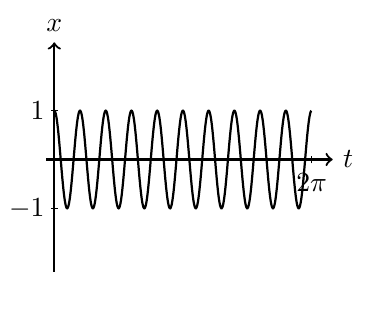
\begin{tikzpicture}[x=0.52cm,y=0.62cm]
    \def\xMax{6.283185}
    \path[use as bounding box]
        (-0.65,-2.5) rectangle (7.3,2.7);

    \draw[->,thick] (-0.2,0) -- (6.8,0)
        node[right] {$t$};
    \draw[->,thick] (0,-2.3) -- (0,2.4)
        node[above] {$x$};

    \draw[thick,domain=0:\xMax,samples=600]
        plot (\x,{cos(deg(10*\x))});

    \foreach \y in {-1,1}{
        \draw (-0.08,\y) -- (0.08,\y);
        \node[left] at (0,\y) {$\y$};
    }
    \draw (\xMax,-0.08) -- (\xMax,0.08);
    \node[below] at (\xMax,-0.08) {$2\pi$};
\end{tikzpicture}
\caption{$\cos10t$}
\end{subfigure}
\hfill
\begin{subfigure}[t]{0.48\linewidth}
\centering
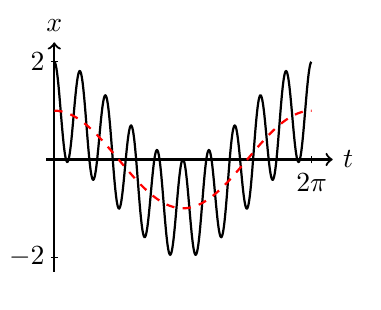
\begin{tikzpicture}[x=0.52cm,y=0.62cm]
    \def\xMax{6.283185}
    \path[use as bounding box]
        (-0.65,-2.5) rectangle (7.3,2.7);

    \draw[->,thick] (-0.2,0) -- (6.8,0)
        node[right] {$t$};
    \draw[->,thick] (0,-2.3) -- (0,2.4)
        node[above] {$x$};

    \draw[thick,domain=0:\xMax,samples=600]
        plot (\x,{cos(deg(10*\x))+cos(deg(\x))});
    \draw[red,dashed,thick,domain=0:\xMax,samples=200]
        plot (\x,{cos(deg(\x))});

    \foreach \y in {-2,2}{
        \draw (-0.08,\y) -- (0.08,\y);
        \node[left] at (0,\y) {$\y$};
    }
    \draw (\xMax,-0.08) -- (\xMax,0.08);
    \node[below] at (\xMax,-0.08) {$2\pi$};
\end{tikzpicture}
\caption{$\cos10t+\cos t$}
\end{subfigure}
\caption{Adding $\cos t$ shifts the fast oscillation
onto a moving centerline (dashed).}
\end{figure}

Next, we consider close but unequal frequencies,
which can produce \textbf{beats}.



%%%%%%%%%%%%%%%%%%%%%%%%%%%%%%%%%%%%
\section{Beats}

\subsection{Close Frequencies}

\paragraph{Desmos experiment.}
On Desmos, plot the function $y=\cos(ax)+\cos(bx)$ with sliders for $a$ and $b$.
Fix $b=30$ and increase $a$ from $1$ to $29$. Observe how the interference pattern changes as the frequency $a$ approaches $b$. The pattern that emerges is called a \textit{beat}.

A \textbf{beat} is a pattern of repeated growth and decline
in amplitude produced by waves with close but unequal
frequencies. Consider the sum
\[
x(t)=\cos(\omega t)+\cos(\omega_0t),
\qquad \omega\approx\omega_0,\quad \omega\ne\omega_0.
\]
The closer the frequencies, the more slowly the amplitude
changes. There is no exact cutoff for ``close.'' For our sketches,
a useful guideline is
\[
\frac{\text{smaller frequency}}{\text{larger frequency}}
\ge 0.8,
\]
with the frequencies unequal. If the frequencies are within $80\%$ of each other, it is fair to call it a beat.

%-------------------------------------------------------------
\subsection{Envelope and Carrier}

There is a useful trig identity for sums of waves
\[
\cos a+\cos b
=2\cos\left(\frac{a+b}{2}\right)
  \cos\left(\frac{a-b}{2}\right).
\]
Applying this to the beat function yields 
\begin{align*}
x(t)&=\cos(\omega t)+\cos(\omega_0t)\\
&=\underbrace{2\cos(\omega_e t)}_{\text{slow factor}}
\underbrace{\cos(\omega_c t)}_{\text{fast factor}},
\end{align*}
where
\[
\omega_e=\frac{|\omega-\omega_0|}{2},
\quad\text{and}\quad
\omega_c=\frac{\omega+\omega_0}{2}.
\]
We call $\omega_e$ the \textbf{envelope frequency}
and $\omega_c$ the \textbf{carrier frequency}.
Close frequencies give $\omega_e\ll\omega_c$. The reason why $\omega_e$ is called the "envelope" frequency is because the curves $\pm2\cos(\omega_e t)$ form the outer layer for the beat function.

%-------------------------------------------------------------
\subsection{Sketching Beats}

To sketch a beat:
\begin{enumerate}
    \item Rewrite the sum or difference as a product.
    \item Draw the positive and negative slow factors
    as dashed envelope curves.
    \item Find the envelope and carrier periods.
    \item Draw the fast oscillation between the envelopes.
\end{enumerate}

%-------------------------------------------------------------
\begin{example}[3]{
Rewrite $x(t)=\cos28t+\cos30t$ as a product and sketch
it, indicating the envelope and its period.
}
The sum-to-product identity gives
\[
x(t)=2\cos(29t)\cos t.
\]
The envelope curves and periods are
\[
x=\pm2\cos t,\qquad
T_e=2\pi,\qquad T_c=\frac{2\pi}{29}.
\]
Thus, the carrier completes $29$ cycles during one
period of the slow cosine. Begin at $x(0)=2$ and
draw the fast oscillation between the dashed curves.

\begin{center}
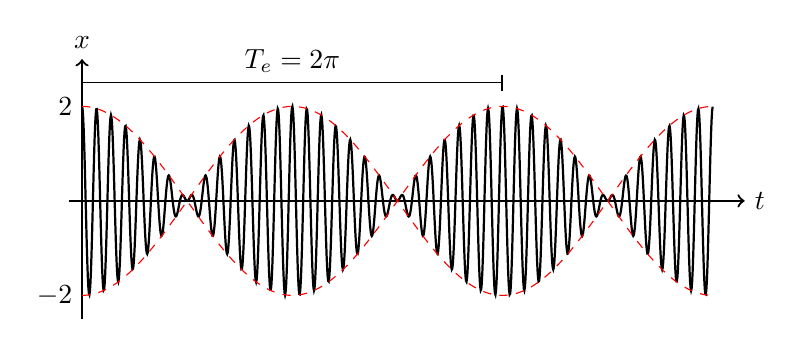
\begin{tikzpicture}[x=0.85cm,y=0.6cm]
    \def\xMax{9.424778}

    \draw[->,thick] (-0.2,0) -- (9.9,0)
        node[right] {$t$};
    \draw[->,thick] (0,-2.5) -- (0,3)
        node[above] {$x$};

    % Full solution
    \draw[thick,domain=0:\xMax,samples=1200]
        plot (\x,{2*cos(deg(\x))*cos(deg(29*\x))});

    % Envelope curves
    \draw[red,dashed,domain=0:\xMax,samples=300]
        plot (\x,{2*cos(deg(\x))});
    \draw[red,dashed,domain=0:\xMax,samples=300]
        plot (\x,{-2*cos(deg(\x))});

    % Period of the slow cosine
    \draw[|-|] (0,2.5) -- ({2*pi},2.5);
    \node[above] at ({pi},2.5) {$T_e=2\pi$};

    \node[left] at (0,2) {$2$};
    \node[left] at (0,-2) {$-2$};
\end{tikzpicture}

\small
Dashed: envelope curves $\pm2\cos t$.
There are $29$ carrier cycles over the marked interval.
\end{center}
\end{example}


% \subsection{Amplitude Modulation and Sound Waves}

% When two tones have close but unequal frequencies,
% their interference makes the sound repeatedly grow
% louder and softer:
% \[
% \text{``waa... waa... waa...''}
% \]
% This variation in amplitude is called
% \textbf{amplitude modulation}. Musicians can use beats
% when tuning an instrument: as a note approaches the
% reference frequency, the beats become slower. 

%%%%%%%%%%%%%%%%%%%%%%%%%%%%%%%%%%%%%%%%%%%%%%%%%%%%%%%%%%%%%%%%%%%%%%%%
\section{Resonance}

\subsection{Matching Frequencies}

Consider an undamped system whose forcing frequency
matches its natural frequency:
\[
x''+\omega_0^2x=F\cos(\omega_0t),
\qquad \omega_0>0,\quad F\ne0.
\]
The usual trial function duplicates the homogeneous
solution, so we multiply it by $t$:
\[
x_p(t)=t\bigl(A\cos(\omega_0t)+B\sin(\omega_0t)\bigr).
\]
Thus, even before determining the coefficients, the
general form of the solution is 
\[
x(t)=
\underbrace{c_1\cos(\omega_0t)+c_2\sin(\omega_0t)}
_{\text{bounded oscillation}}
+
\underbrace{t\bigl(A\cos(\omega_0t)+B\sin(\omega_0t)\bigr)}
_{\text{growing oscillation}}.
\]
The factor $t$ produces unbounded growth despite the
bounded forcing. This is \textbf{resonance} in the
undamped model. The bounded homogeneous part cannot
cancel this growth. 

%-------------------------------------------------------------
\subsection{Recognizing Resonance}

For unbounded resonance, we require no damping. Next, we must sinusoidal forcing term
\[
mx''+kx=F_0\cos(\omega t)
\quad\text{or}\quad
mx''+kx=F_0\sin(\omega t).
\]
Lastly, the innate frequency of the system $\sqrt{\frac{k}{m}}$must match the forcing frequency
\[
\boxed{\omega=\sqrt{\frac{k}{m}}=\omega_0.}
\]
These are the key requirements for a forced vibration to exhibit resonance. 

\begin{example}[4]{
An undamped spring has stiffness $k=12$ N/m and is
driven by the force $f(t)=10\sin6t$ N.
What mass produces resonance?
}
The model is
\[
mx''+12x=10\sin6t.
\]
Matching the natural and forcing frequencies gives
\[
\sqrt{\frac{12}{m}}=6
\implies \frac{12}{m}=36
\implies \boxed{m=\frac13\text{ kg}.}
\]
\end{example}

We can distinguish resonance, beats, and ordinary
interference by comparing the natural and forcing frequencies.

\begin{example}[5]{
Classify the expected behavior as \textbf{resonance},
\textbf{beats}, or \textbf{ordinary interference}.
For unequal frequencies, assume both wave components
are present with comparable amplitudes.
\begin{enumerate}
    \item $x''+4x=\cos t$
    \item $x''+49x=2\cos50t$
    \item $x''+64x=\sin7t$
    \item $2x''+8x=4\sin2t$
\end{enumerate}
}
First identify $\omega_0=\sqrt{k/m}$ and the forcing
frequency $\omega$. Equal frequencies give resonance.
For unequal frequencies, use our $80\%$ guideline
to recognize beats:
\[
r=\frac{\min(\omega_0,\omega)}{\max(\omega_0,\omega)}.
\]

\begin{center}
\renewcommand{\arraystretch}{1.3}
\begin{tabular}{c|c|c|c|l}
Equation & $\omega_0$ & $\omega$ & $r$ & Behavior\\
\hline
1 & $2$ & $1$ & $0.50$ & Ordinary interference\\
2 & $7$ & $50$ & $0.14$ & Ordinary interference\\
3 & $8$ & $7$ & $0.875$ & Beats\\
4 & $2$ & $2$ & $1$ & Resonance
\end{tabular}
\end{center}

In equation 4, divide by $2$ first:
\[
x''+4x=2\sin2t.
\]
Thus, $\omega_0=2=\omega$, so the response is resonant.

Beats are also an interference pattern; the close
frequencies produce a slowly varying amplitude.
\end{example}

%%%%%%%%%%%%%%%%%%%%%%%%%%%%%%%%%%%%%%%%%%%%%%%%%%%%%%%%%%%%%%%%%%%%%%%%
\section{Connections to Sound and Other Waves}

\subsection{Sound Waves}

At a fixed location, a pure sound tone can be modeled
by an oscillating pressure:
\[
p(t)=A\cos(\omega t).
\]
The frequency $\omega$ determines the pitch, while the amplitude $A$
affects the loudness. Here, $\omega$ is measured in
radians per second; the frequency in hertz is
$f=\omega/(2\pi)$.

Suppose two speakers play different tones simultaneously.
Each produces its own pressure variation:
\[
p_1(t)=A_1\cos(\omega_1t),
\qquad
p_2(t)=A_2\cos(\omega_2t).
\]
At the listener's position, these variations add:
\[
p(t)=p_1(t)+p_2(t)
=A_1\cos(\omega_1t)+A_2\cos(\omega_2t).
\]
For simplicity, we have chosen zero phase shifts.
The resulting pressure is the combined sound that
reaches the listener's ear.

This is the same \textbf{interference} we studied earlier:
the waves reinforce one another when their pressure
variations have the same sign and partially or completely
cancel when they have opposite signs.
%-------------------------------------------------------------
\subsection{Hearing Beats}

\paragraph{Tuning a piano.}
A tuning fork produces a reference tone, and striking
a piano key produces another tone. When played together,
their sound waves add. If the piano is perfectly tuned
to the fork, we hear a steady tone without beats.
If it is slightly out of tune, the waves move into
and out of step. The sound grows louder and softer:
``waa... waa... waa...''
These pulses are called \textbf{beats}.
As the piano's frequency approaches the fork's frequency,
the beats slow down and eventually disappear.
This lets the tuner hear when the note is in tune.

\paragraph{AM radio.}
A changing amplitude can also carry information.
In \textbf{amplitude modulation} (AM), a transmitter
varies the amplitude of a fast carrier wave according
to the speech or music being broadcast:
\[
p(t)=\bigl(A+s(t)\bigr)\cos(\omega_c t),
\qquad A>|s(t)|.
\]
Here, $s(t)$ is the audio signal and $p(t)$ is the
electrical signal sent to the antenna. The high-frequency
carrier allows efficient transmission, while its changing
amplitude carries the sound. Different stations use
different carrier frequencies, allowing your radio
to select one station and recover its audio.
%-------------------------------------------------------------
\subsection{Resonance and Its Applications}

\paragraph{Pushing a swing.}
A playground swing has a natural rhythm. If you time your kicks
to match that rhythm, each push adds energy and the
swing goes higher. This illustrates resonance:
a repeated force reinforces the motion when applied
at the right frequency. Friction and air resistance
keep a real swing from growing without limit.

\paragraph{Shattering a wine glass.}
Tapping a wine glass makes it ring at one of its natural
frequencies. A singer who sustains a matching pitch can
drive that vibration through the pressure of the sound.
If the sound is sufficiently intense and the glass
has little damping, the vibration can become large
enough to shatter it. If you've seen old cartoons of people breaking glass with their voice, that is an example of resonance.

\paragraph{The Tacoma Narrows Bridge.}
Structures such as bridges have natural frequencies
at which they tend to vibrate. In 1940, wind caused
increasingly large twisting motions in the Tacoma
Narrows Bridge until it collapsed. This is often
presented as resonance: the wind supposedly matched
the bridge's natural frequency.

However, the main mechanism is now believed to be \textit{flutter}!
As the bridge twisted, it changed the airflow.
The wind then reinforced the twisting, making the
motion grow. Unlike our model, the force depended
on the bridge's own motion.

\paragraph{Magnetic resonance imaging (MRI).}
MRI uses resonance to take pictures inside the body.
A strong magnet and carefully tuned radio waves cause
hydrogen nuclei in the body to respond and produce
signals. The scanner detects these signals and uses
them to build images of organs and other tissues.
The key idea is familiar: choosing the right frequency
makes the system respond.
\end{document}